We were mainly interested in answering two questions:

\begin{enumerate}

  \item how far in the future can our system predict well?

  \item how does the knowledge of the grasped object affect the error?

\end{enumerate}

In order to answer the first question, we have checked how the error
on regression changes as $B$ varies from $0.1$ to $0.5$. This
procedure was repeated independently for each single sensor.

To obtain statistically meaningful results, we recorded each mean
error obtained \emph{on a single fold} of the cross-validation
procedure; for each sensor and value of $B$, this means we have
obtained $5$ numbers. The errors for each sensor were then grouped
accordingly to their measurement units and meaning: the position of
the hand ($3$ sensors, the $x,y,z$ from the FoB), the hand orientation
($3$ sensors, the azimuth, elevation and roll from the FoB), and the
posture of the hand ($22$ sensors, the joint positions from the
CyberGlove). According to the device resolutions (see the previous
Section), we set $\epsilon$ to $0.1$ inches for the hand position,
$0.5$ degrees for the hand orientation and $1$ degree for the hand
posture.

Lastly, for each group of sensors, we averaged the errors \emph{per
single cross-validaton fold}, and evaluated the mean and standard
deviation of the resulting $5$ values. This gave us an indication of
how well our machine performed on the hand position, orientation and
posture. In all graphs, the points on the curves represent the mean
values, whereas the error bars are placed at $\pm 1$ standard
deviations which is common practice in machine learning. 

In order to answer the second question, we first evaluated the error
obtained as described above using all sessions for each single object,
so to obtain an estimate of how complex it is to approximate the grasp
for the can, roll and mug unbiased by the differences among the
subjects. Subsequently we averaged these three errors and compared the
averages with the overall error, obtained by joining \emph{all}
sessions together in a single training set.

\subsection{Prediction power}

%Figure \ref{fig:err_all} shows the main experimental results.

\begin{figure}[htbp]
  \begin{center}
    \begin{tabular}{cc}
      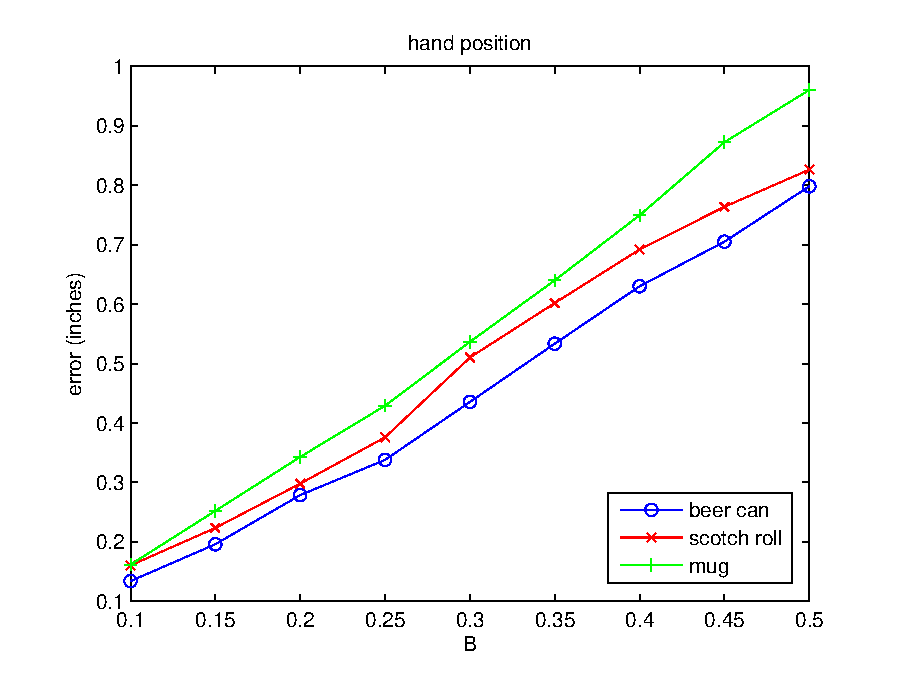
\includegraphics[width=0.45\textwidth]{error_pos.eps} &
      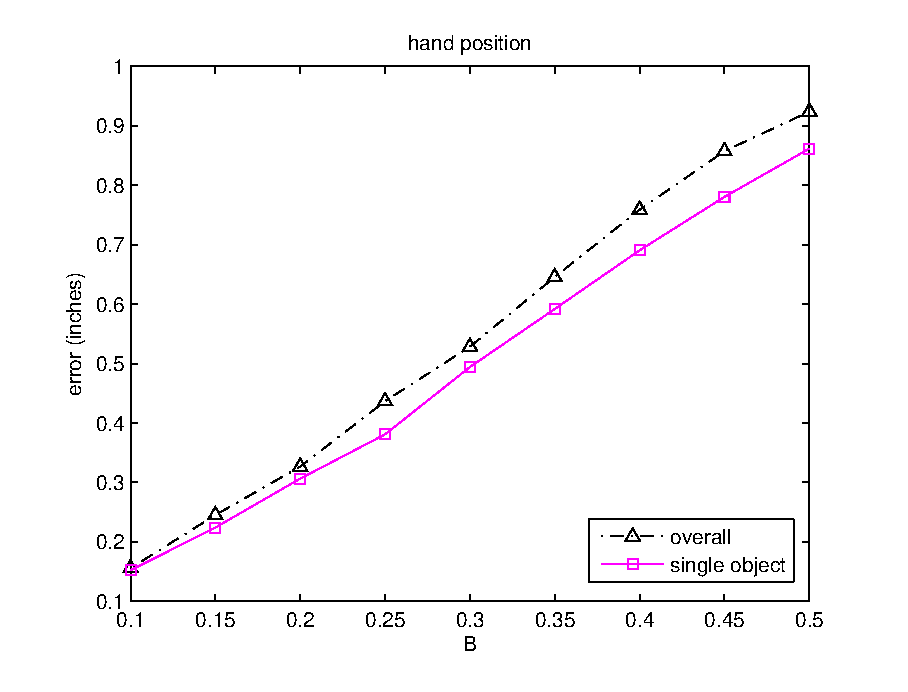
\includegraphics[width=0.45\textwidth]{error_cmp_pos.eps} \\
      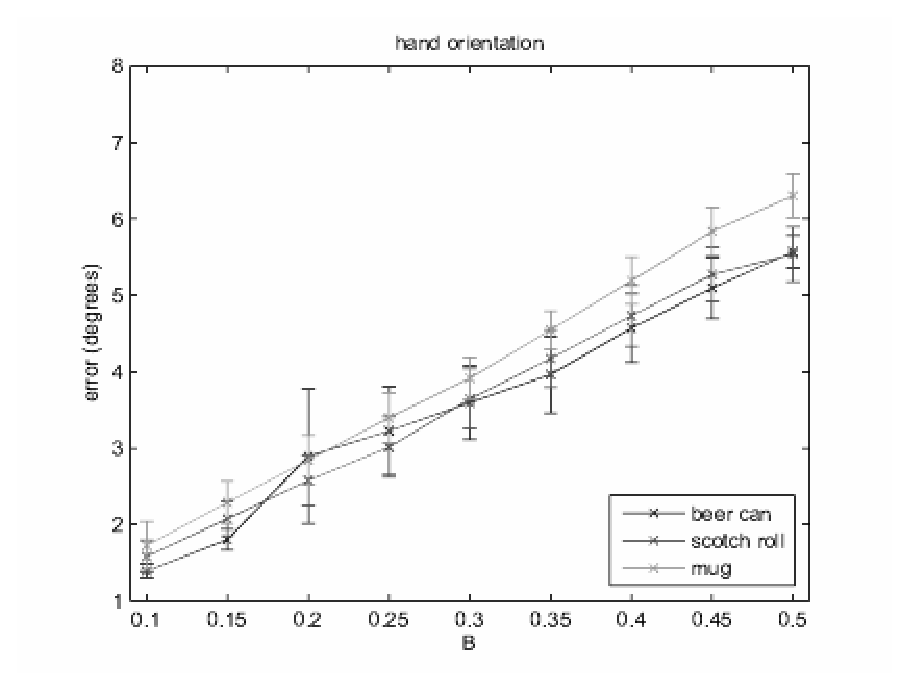
\includegraphics[width=0.45\textwidth]{error_ori.eps} &
      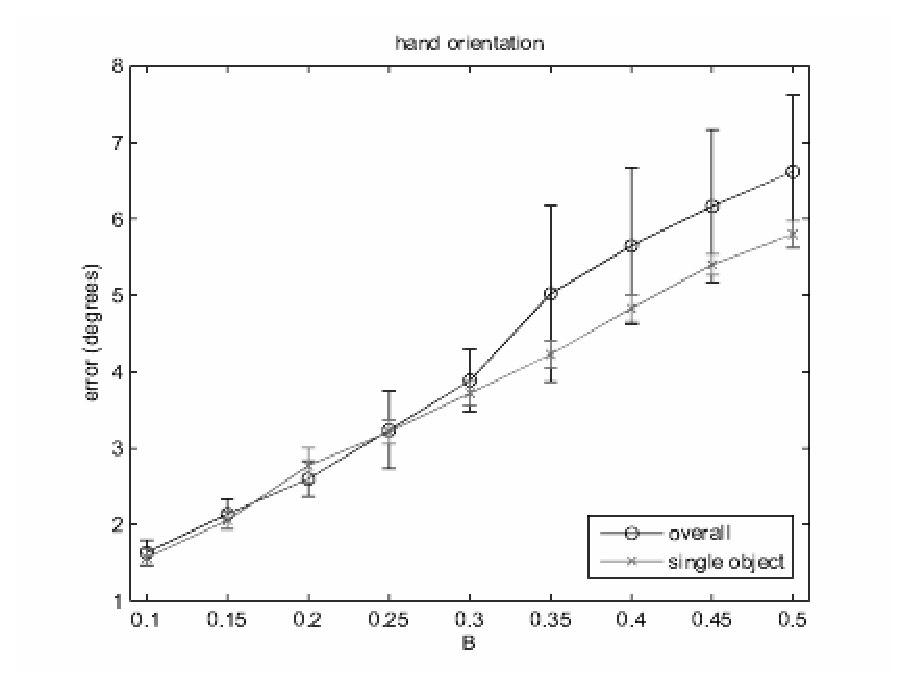
\includegraphics[width=0.45\textwidth]{error_cmp_ori.eps} \\
      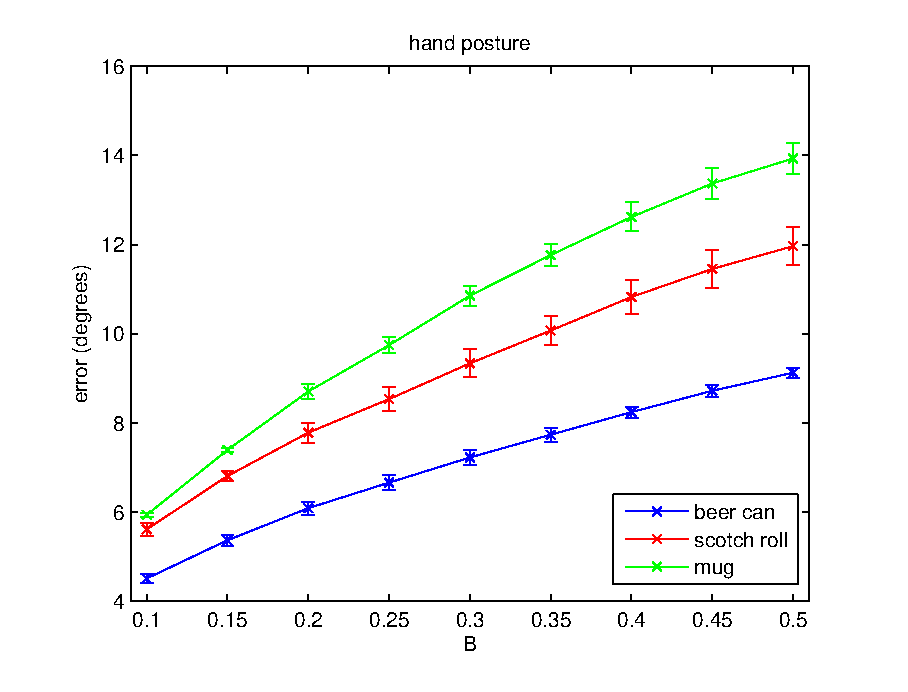
\includegraphics[width=0.45\textwidth]{error_pst.eps} &
      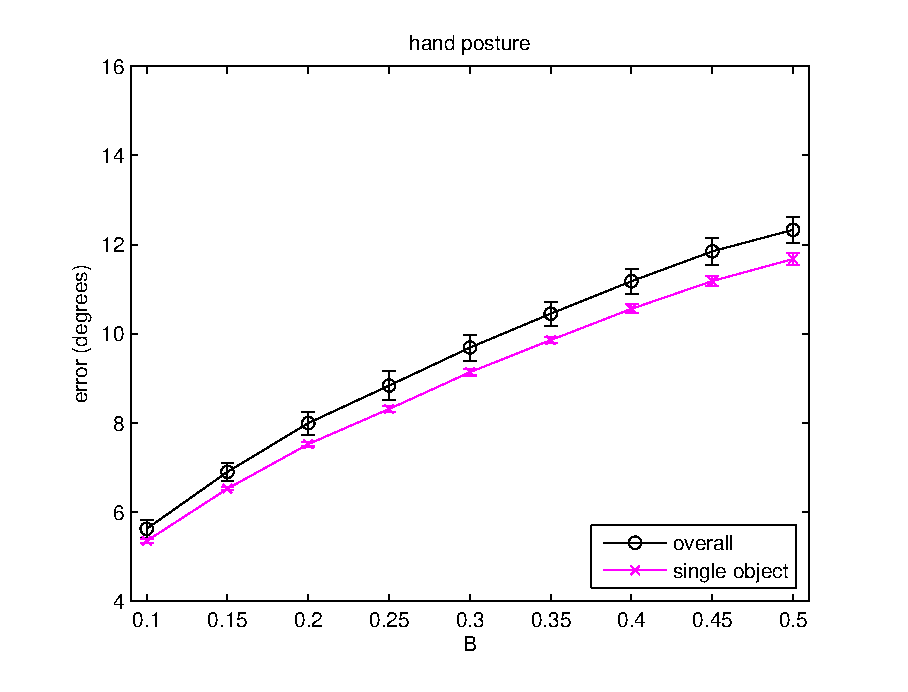
\includegraphics[width=0.45\textwidth]{error_cmp_pst.eps} \\
    \end{tabular}
    \caption{Regression results as the blind fraction $B$ increases
    from $0.1$ to $0.5$. In each row the
    left-hand side pictures compare the errors on different objects,
    while the right-hand side pictures compare the average error on
    single objects and the overall error.}
    \label{fig:err_all}
  \end{center}
\end{figure}

With reference to Figure \ref{fig:err_all}, left column: first of all, as $B$
increases, the error does, as it was intuitively expected: the more
data is hidden, the harder the prediction becomes. Then, as one can
see, as far as the hand position and orientation are concerned, the
three objects show comparable errors. On the other hand, there is a
precise ranking in the hand posture regression: the mug is more
difficult than the scotch roll, which is in turn harder than the beer
can. This also is intuitively sensible, since it is possible to grasp
the scotch roll in more ways than the can, and it is possible to grasp
the mug in even more ways (especially, using the handle).

The analysis of the obtained models (see Figure
\ref{fig:hyperp}, left column) shows that, accordingly, the percentage
of Support Vectors with respect to the total number of samples
increases steadily as $B$ grows, indicating that the problem becomes
harder and harder. The three curves also confirm that regression on
the mug is the most difficult, followed in turn by the scotch roll and
the beer can.

\begin{figure}[htbp]
  \begin{center}
    \begin{tabular}{cc}
      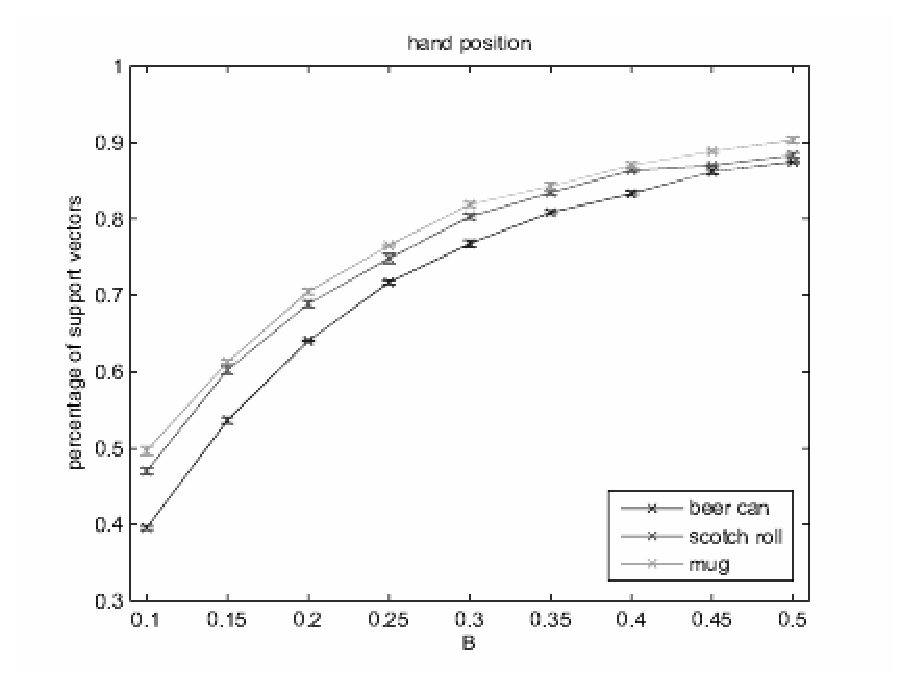
\includegraphics[width=0.45\textwidth]{error_pos_SV.eps} &
      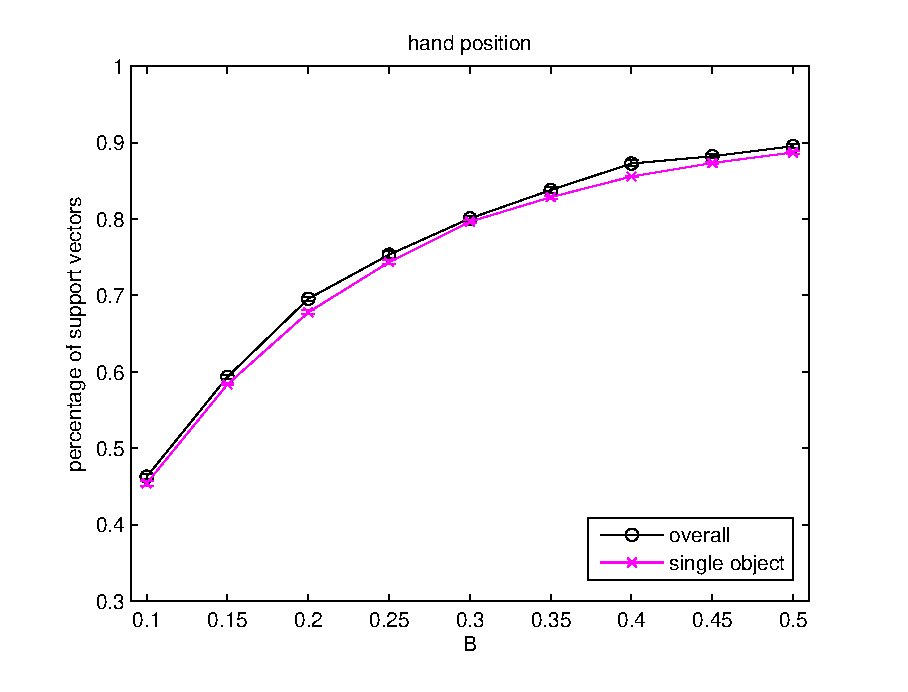
\includegraphics[width=0.45\textwidth]{error_cmp_pos_SV.eps} \\
      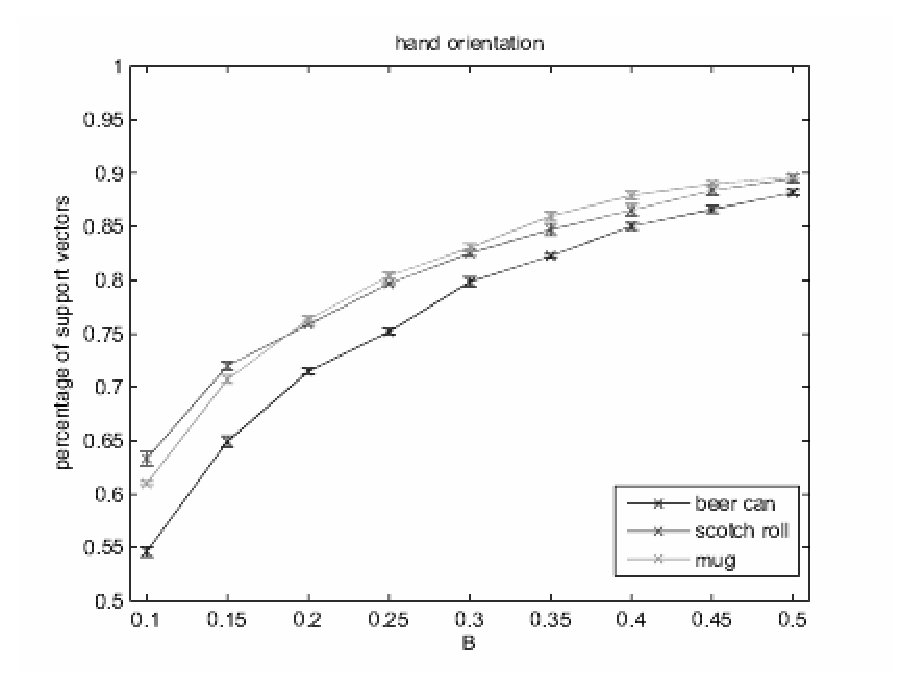
\includegraphics[width=0.45\textwidth]{error_ori_SV.eps} &
      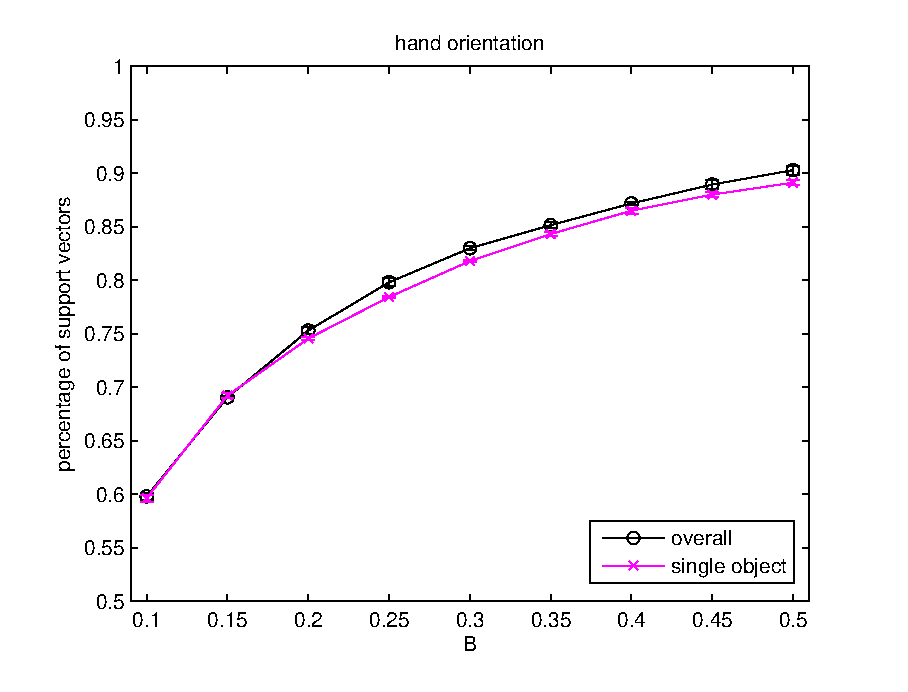
\includegraphics[width=0.45\textwidth]{error_cmp_ori_SV.eps} \\
      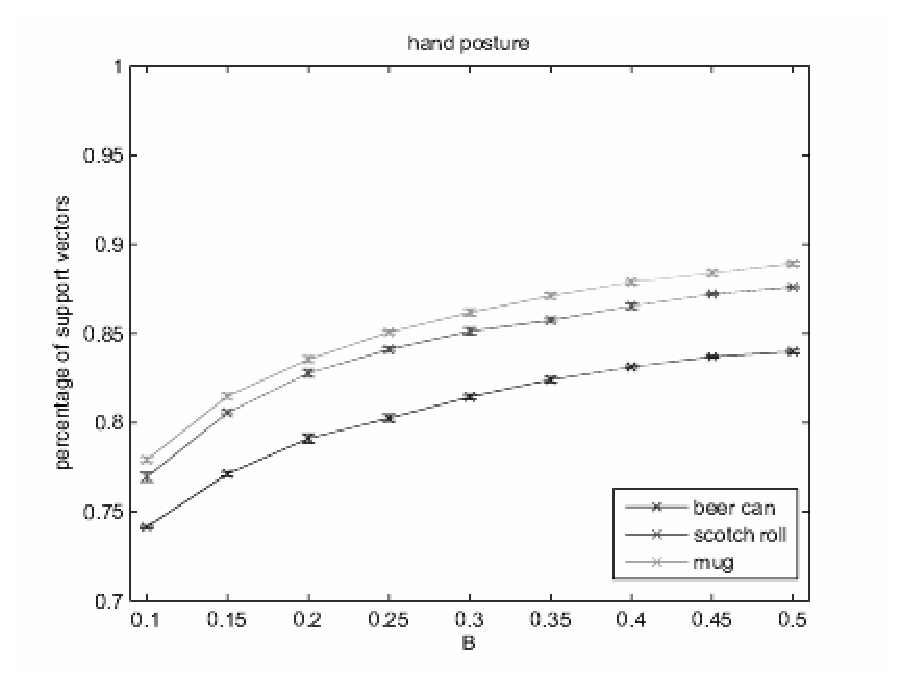
\includegraphics[width=0.45\textwidth]{error_pst_SV.eps} &
      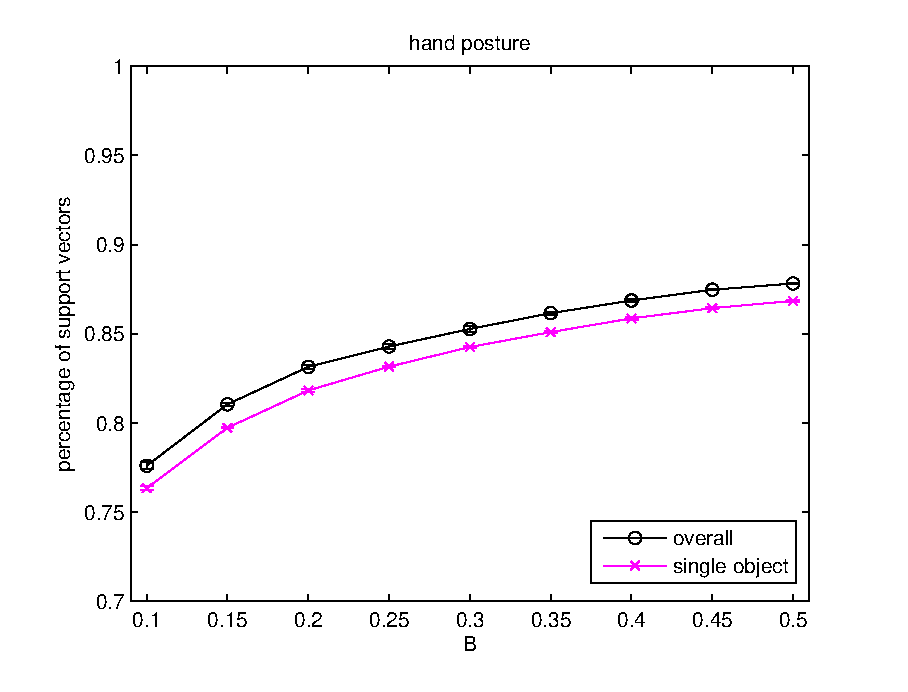
\includegraphics[width=0.45\textwidth]{error_cmp_pst_SV.eps} \\
    \end{tabular}
    \caption{Percentage of support vectors with respect to the total
    number of samples.}
    \label{fig:hyperp}
  \end{center}
\end{figure}

A further analysis of the hyperparameters (see Figure
\ref{fig:C_trend}) confirms that, as $B$ increases, more and more
information is missing from the training set: both $C$ and $\sigma$
show a decreasing trend on all three groups of sensors (more
pronounced in the case of $C$), meaning that the regularisation term
in Equation (\ref{eqn:svm_primal}) becomes more and more important,
and that the Gaussians used to build the solution become narrower and
narrower.

\begin{figure}[htbp]
  \begin{center}
    \begin{tabular}{cc}
      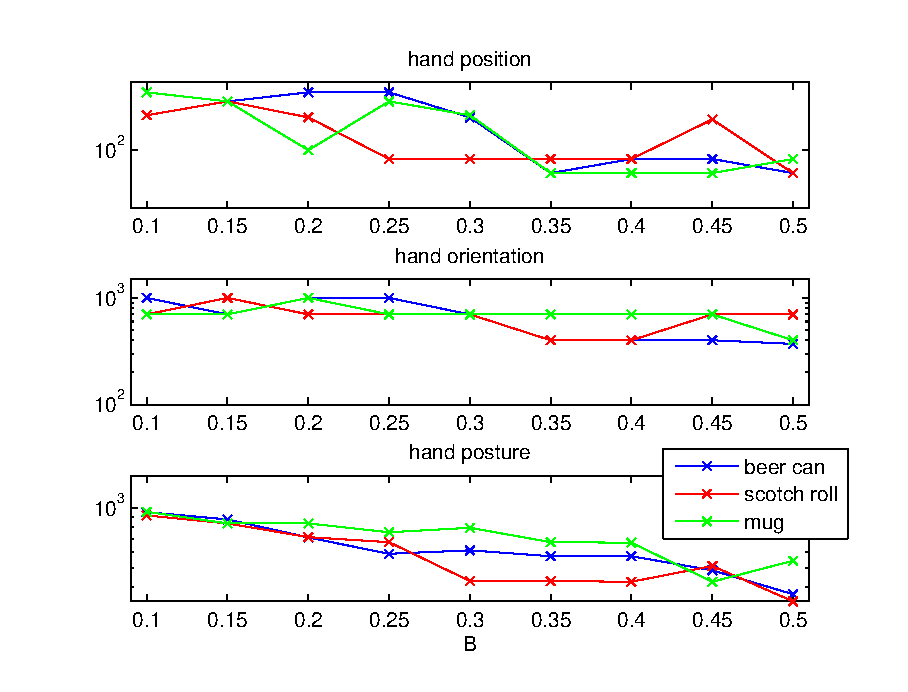
\includegraphics[width=0.45\linewidth]{trend_C.eps} &
      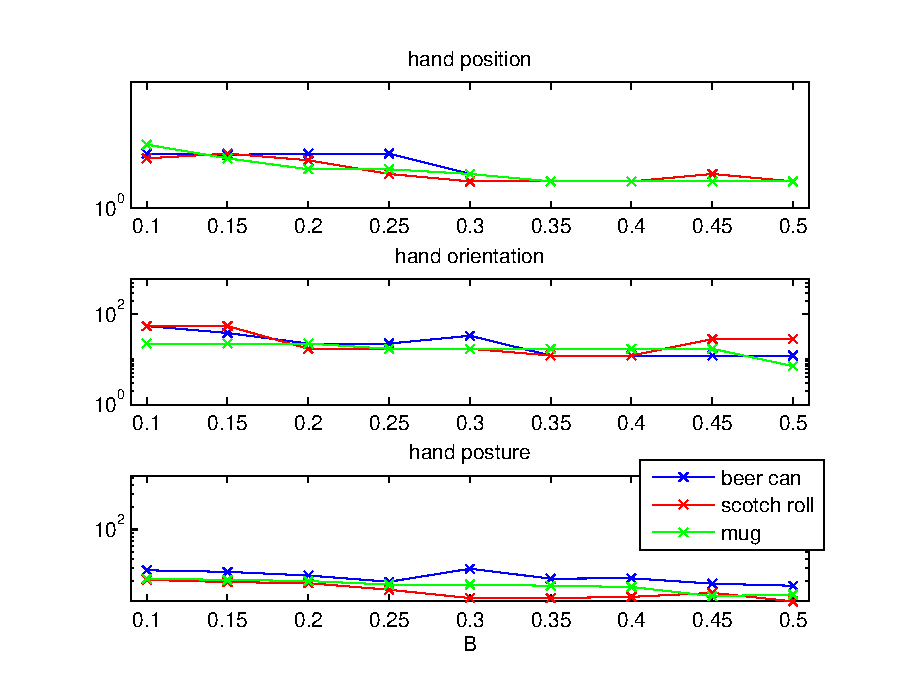
\includegraphics[width=0.45\linewidth]{trend_sigma.eps}
    \end{tabular}
    \caption{The trend of the hyperparameters $C$ (left pane) and
    $\sigma$ (right pane), as far as the hand position, orientation
    and posture is concerned. As $B$ is increased, both parameters show a
    decreasing trend, more pronounced in the case of $C$.}
    \label{fig:C_trend}
  \end{center}
\end{figure}

To determine how far in the future SVMs can predict well, we need to
decide what an acceptable error is. In general, this is
application-dependent. In this case we decided to accept an error as
large as $5$ times a minimum threshold, determined by taking into
account the resolutions of the sensors as declared in the devices
manuals and related publications (see the previous Section). This lead
us to $0.5$ inches for the hand position, $2.5$ degrees for the hand
orientation, and $7.5$ degrees for the hand posture. As far as the
hand posture is concerned, it must be remarked that, in this paper, we
have only considered the average of errors on all the $22$ sensors,
whereas in a more detailed analysis one should take into account that,
e.g., an error on the wrist pitch would lead to a worse displacement
of the hand, than an error on a phalanx would. This is subject of
future research.

As one can see from the graphs, the acceptable error is attained for
the hand position at $B=0.3$, for the hand orientation at $B=0.2$ and
for the hand posture at $B=0.15$ (mug), $0.2$ (scotch roll) and
$B=0.35$ (beer can). Since the average grasp lasts on average $0.62$
seconds, we can say that the system can predict reasonably well

\begin{itemize}

  \item something less than $200$ milliseconds in advance the hand
    position,

  \item about $120$ milliseconds in advance the hand orientation, and

  \item about $100-200$ milliseconds in advance the hand posture, the
    mug being the hardest and the beer can the easiest object.

\end{itemize}

This answers the first question.

\subsection{Knowledge of the objects}

As far as the second question is concerned, consider Figure
\ref{fig:err_all}, right column: the curve representing the error on
the single objects is basically always smaller than the other one,
indicating that a specific SVM trained on a single object will on
average be more precise than a SVM trained on all objects altogether:
the \emph{a priori} knowledge of the object improves the
performance.

Notice that this effect is more pronounced in the case of the hand
posture than for the hand position and orientation, where a
substantial overlap of the error bars can be seen (the ANOVA test on
the error indicates no significance for the hand position and
orientation, but high significance for the posture ($p<0.01$)). This is sensible,
since knowing \emph{what object} one is going to grasp will tell a
great deal about \emph{how to shape one's hand} in order to grasp it,
but it will definitely be less influential in order to determine where
and how to \emph{reach} unless there is a strong connection between
the grasp type and the wrist orientation.

Let us now focus upon the fraction of SVs found by the SVMs: consider
Figure \ref{fig:hyperp}, right column. It turns out that SVMs trained
on single objects have a \emph{definitely smaller} fraction of SVs
than the one trained on the overall sequence. This means that the
machines trained on single objects \emph{are smaller and simpler than
the overall one, while being more precise.}

Summing up, we can say that if the problem is split into subproblems,
each one regarding a single object, performances are better and the
computational complexity is smaller. This phenomenon is particularly
evident as far as the hand posture is concerned, as one can
intuitively expect.

This answers the second question.

\subsection{Single grasp types}

A further interesting question is:

\begin{itemize}

  \item how well does our system perform on \emph{specific types of
    grasps}?

\end{itemize}

In order to shed light on this point, we have considered the most
complex and interesting object under this point of view, i.e., the
mug. All sessions in which the subjects were grasping the mug have
been collected, and all final grasping hand postures have been
considered as representing the ways the mug was grasped. This resulted
in slightly more than $2550$ samples, according to the fact that each
of the $11$ subjects performed about $240$ mug grasps.

The final positions were then clustered using a K-means clustering
algorithm (see, e.g., \cite{macqueen}). We used the freely available
\emph{Fuzzy Clustering and Data Analysis} Matlab toolbox
\cite{fctBalasko1,fctBalasko2}; due to the intrinsically stochastic
nature of the algorithm, we ran the algorithm $100$ times for
$1,\ldots,10$ clusters and employed Dunn's Index \cite{dunn} to
determine what was the optimal number of clusters. It was determined
that the optimal number of clusters was $4$.
%% , corresponding to the four
%% hand postures visible in Figure \ref{fig:postures}.

%% \begin{figure}[htbp]
%%   \begin{center}
%%     \begin{tabular}{cccc}
%%       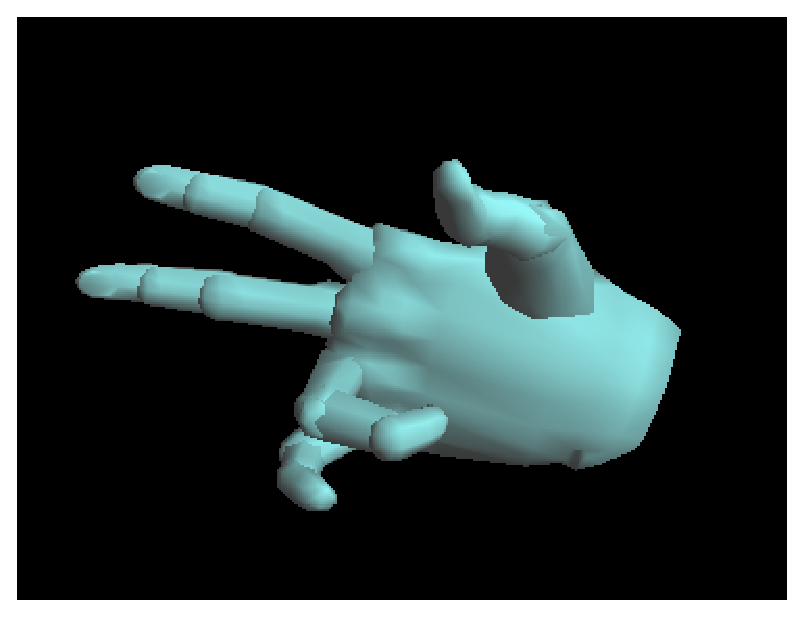
\includegraphics[width=0.22\linewidth]{posture1.eps} &
%%       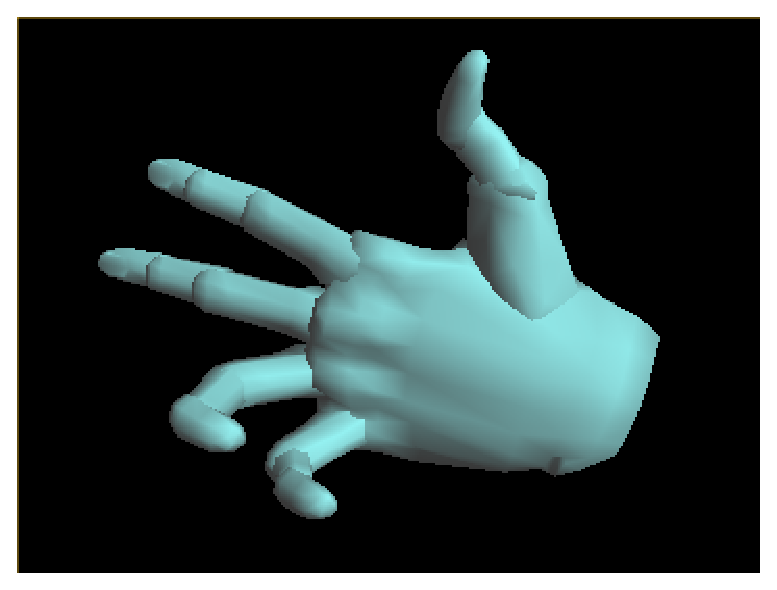
\includegraphics[width=0.22\linewidth]{posture2.eps} &
%%       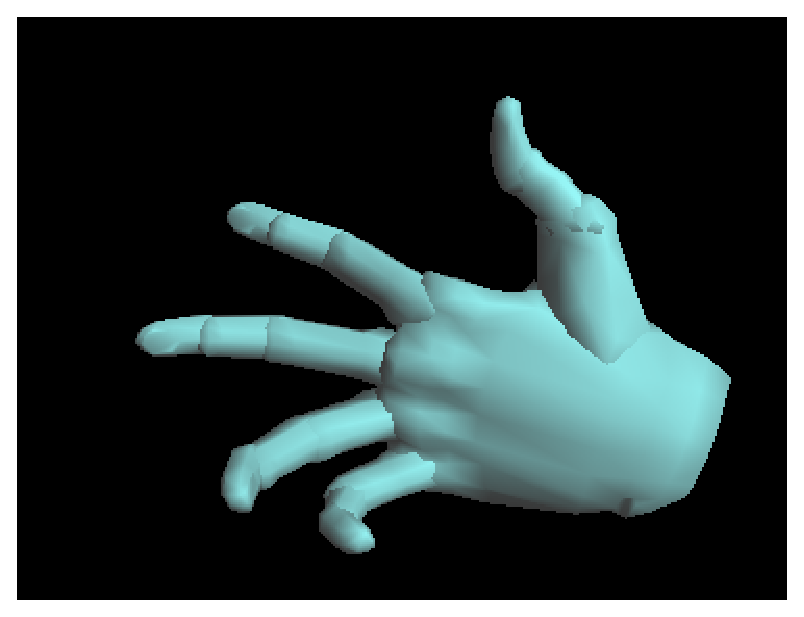
\includegraphics[width=0.22\linewidth]{posture3.eps} &
%%       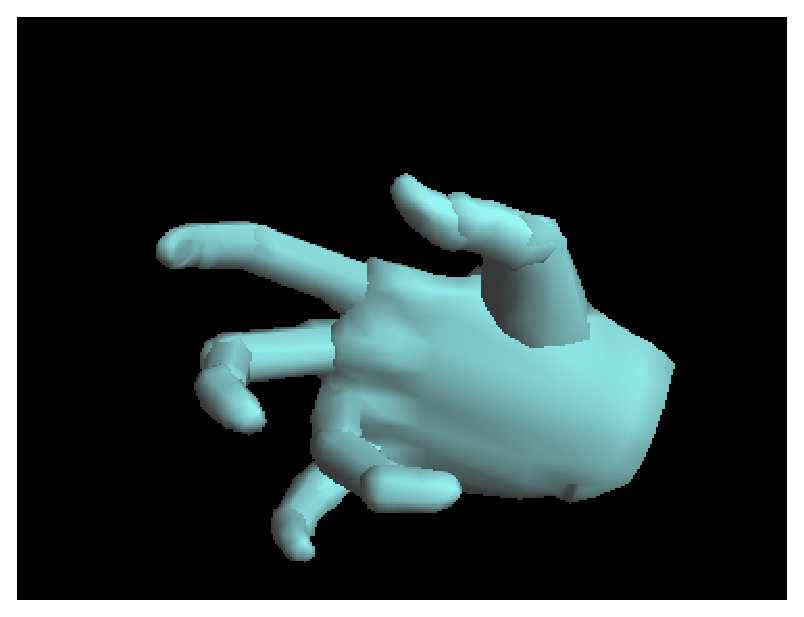
\includegraphics[width=0.22\linewidth]{posture4.eps} \\
%%       (1) & (2) & (3) & (4) \\
%%     \end{tabular}
%%     \caption{The four prototypical hand postures when grasping the
%%       mug, as found by K-means clustering.}
%%     \label{fig:postures}
%%   \end{center}
%% \end{figure}

We then split the mug grasps into four sets according to the
clustering, and ran separate experiments on each set for
$B=0.1,\ldots,0.5$; the four clusters represent about one quarter each
of the total mug grasps. Lastly, we compared the four error and SV
percentage curves to one another, and to the mug curve of Figures
\ref{fig:err_all} and \ref{fig:hyperp}, left column, bottom graph. We
hoped to get more insight on how the knowledge of what grasp is being
examined changed the situation. Figure \ref{fig:clustering} shows the
experimental results.

\begin{figure}[htbp]
  \begin{center}
    \begin{tabular}{cc}
      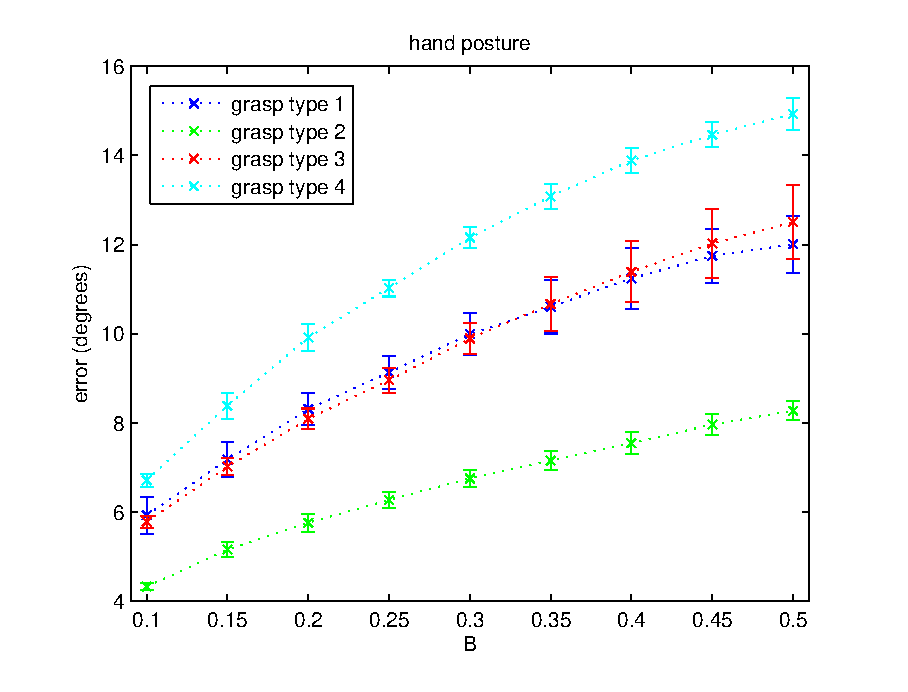
\includegraphics[width=0.45\textwidth]{error_pst_cluster.eps} &
      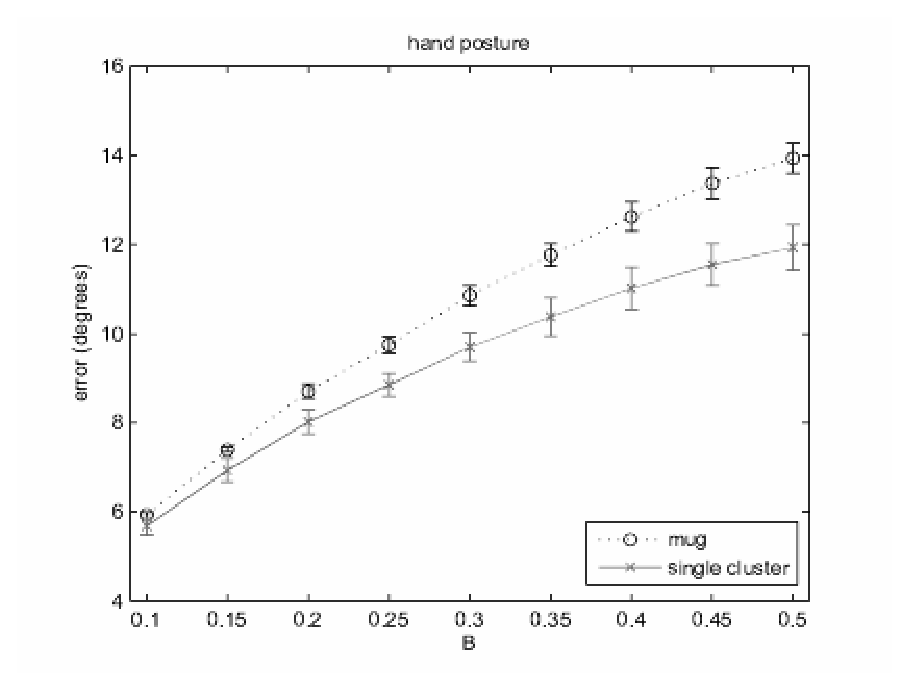
\includegraphics[width=0.45\textwidth]{error_pst_cmp_cluster.eps} \\
      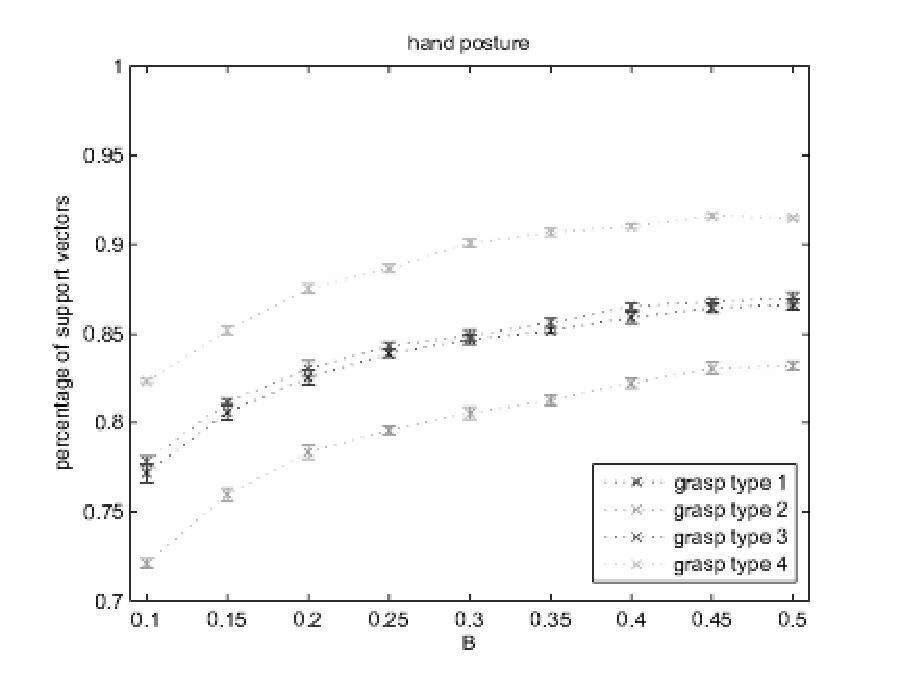
\includegraphics[width=0.45\textwidth]{error_pst_SV_cluster.eps} &
      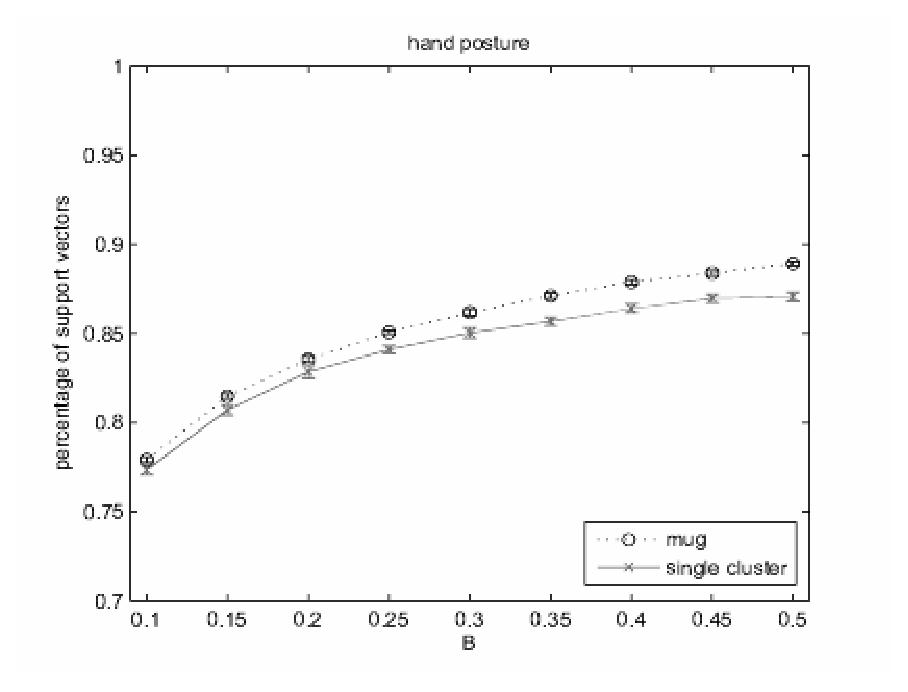
\includegraphics[width=0.45\textwidth]{error_pst_cmp_SV_cluster.eps} \\
    \end{tabular}
    \caption{Comparison among regression on single grasp types (left
      column) and between regression with/without knowledge of the grasp
      type (right column).}
    \label{fig:clustering}
  \end{center}
\end{figure}

First of all, it must be noticed (left column) that there is a
considerably different error among the types of grasps, type $4$ being
the more complex, followed by $1$ and $3$ having the same complexity,
and $2$ being the easiest one. This ranking is confirmed by the
percentage of SVs graph (bottom left). But, as well, the error on the
single grasps is \emph{smaller} than that on the mug in three cases
out of four, and only slightly larger in the case of grasp type
$4$. This suggests that the machine is able to learn well a number of
different grasp types, without ``specialising'' on one easy type.

Secondly, consider Figure \ref{fig:clustering}, right column, showing
an analogous comparison as that shown in Figure \ref{fig:err_all},
right column: in that case we compared the errors obtained with and
without prior knowledge of the object to be grasped; here we compare
the errors \emph{on the mug}, with and without prior knowledge of
\emph{the type of grasp}. The result is that knowing in advance the
type of grasp makes the machine even more accurate and smaller than it
used to be before.
